\documentclass[12pt]{article}
\usepackage[top=1in,left=1in, right = 1in, footskip=1in]{geometry}

\title{Complete characterization of the MERS-Cov outbreak in South Korea using Bayesian latent variable modeling}
\author{Sang Woo Park and Jonathan Dushoff and ?}

\usepackage{graphics}
\usepackage{adjustbox}

\newcommand{\eref}[1]{(\ref{eq:#1})}
\newcommand{\fref}[1]{Fig.~\ref{fig:#1}}
\newcommand{\Fref}[1]{Fig.~\ref{fig:#1}}
\newcommand{\sref}[1]{Sec.~\ref{#1}}
\newcommand{\frange}[2]{Fig.~\ref{fig:#1}--\ref{fig:#2}}
\newcommand{\tref}[1]{Table~\ref{tab:#1}}
\newcommand{\tlab}[1]{\label{tab:#1}}

\usepackage{amsthm}
\usepackage{amsmath}
\usepackage{amssymb}
\usepackage{amsfonts}

\usepackage{hyperref}
\usepackage{natbib}
\usepackage{hyperref}
\bibliographystyle{chicago}
\date{\today}

\usepackage{xspace}
\newcommand*{\ie}{i.e.\@\xspace}

\usepackage{color}

\newcommand{\Rx}[1]{\ensuremath{{\mathcal R}_{#1}}} 
\newcommand{\Ro}{\Rx{0}}
\newcommand{\RR}{\ensuremath{{\mathcal R}}}
\newcommand{\Rhat}{\ensuremath{{\hat\RR}}}
\newcommand{\tsub}[2]{#1_{{\textrm{\tiny #2}}}}

\newcommand{\comment}[3]{\textcolor{#1}{\textbf{[#2: }\textsl{#3}\textbf{]}}}
\newcommand{\jd}[1]{\comment{cyan}{JD}{#1}}
\newcommand{\swp}[1]{\comment{magenta}{SWP}{#1}}
\newcommand{\hotcomment}[1]{\comment{red}{HOT}{#1}}

\begin{document}
\maketitle

\section*{Outline}

It is difficult to infer generation-interval distributions because we often do not have accurate information on key epidemiological dates.
For example, we may have information on when an individual was exposed to potential sources of infections but may not know when that individual was actually infected.
We can overcome this problem by modeling such dates as latent variables.
Here, we outline a statistical model that allows us to handle missing data and infer generation intervals using incomplete contact tracing data.
We apply this method to MERS-Cov outbreak from Korea, where we have reliable information on every patient but not on their contact networks or infection times. 

Here, we're going to use MERS-Cov data set from the \texttt{outbreaks} package from \texttt{R}.
The data set contains a line list (patient-level information) and a partially observed contact tracing data.
The line list contains date of first exposure, date of last exposure, date of sympton onset, and date of report (and several other things we don't really need at this point).
In the package description, it says ``This dataset is meant for teaching purposes; it represents neither the final outbreak investigation results nor a consolidated and complete description of the transmission chain.''
So we can plan our analysis with this data set and apply it to a real data set later on.

Date of report is perfectly known but we have some missing data for other dates.
So we want to use date of report as our reference.
If date of onset is unknown, we sample date of onset uniformly between date of first exposure (set to date of symptom onset of the primary infector, if unknown) to date of report.
Then, we model length of reporting period (difference bewteen date of report and date of onset) as an exponential distribution:
\begin{equation}
t_{i, \tiny{\textrm{rep}}} \sim \mathrm{Exponential}(\lambda_{\tiny\textrm{rep}}),
\end{equation}
where $t_{i, \tiny\textrm{rep}}$ represents either observed or estimated reporting period.
We use exponential distribution to allow for zero because several cases were reported immediately after symptom onset.
Rate parameter $\lambda_{\tiny\textrm{rep}}$ is given an exponential prior with rate of 1:
\begin{equation}
\lambda_{\tiny\textrm{rep}} \sim \mathrm{Exponential}(1).
\end{equation}

Similarly, we draw infection date uniformly from date of first exposure to date of last exposure (set to date of onset, if unknown) and model infectious period (difference between date of onset and date of infection) using a gamma distribution:
\begin{equation}
t_{i, \tiny{\textrm{onset}}} - t_{i, \tiny{\textrm{inf}}} \sim \mathrm{Gamma}(\alpha_{\tiny{\textrm{inf}}}, \beta_{\tiny{\textrm{inf}}}),
\end{equation}
where the shape $\alpha_{\tiny{\textrm{inf}}}$ and rate $\beta_{\tiny{\textrm{inf}}}$ parameters are given independent gamma priors:
\begin{equation}
\begin{aligned}
\alpha_{\tiny{\textrm{inf}}} &\sim \mathrm{Gamma}(4, 2)\\
\beta_{\tiny{\textrm{inf}}} &\sim \mathrm{Gamma}(4, 10)\\
\end{aligned}
\end{equation}
This corresponds to prior mean infectious period of 6.9 days (95\% quantile: 1.1 - 25.5).

For individuals whose infectors are known, generation intervals are calculated by taking the difference between the date of infection of the patient and the date of infection of the infector.
Then, the generation-interval distribution is modeled using a gamma distribution:
\begin{equation}
t_{i, \tiny{\textrm{gen}}} \sim \mathrm{Gamma}(\alpha_{\tiny{\textrm{gen}}}, \beta_{\tiny{\textrm{gen}}}),
\end{equation}
where the shape $\alpha_{\tiny{\textrm{gen}}}$ and rate $\beta_{\tiny{\textrm{gen}}}$ parameters are given independent gamma priors:
\begin{equation}
\begin{aligned}
\alpha_{\tiny{\textrm{gen}}} &\sim \mathrm{Gamma}(4, 2)\\
\beta_{\tiny{\textrm{gen}}} &\sim \mathrm{Gamma}(4, 20)\\
\end{aligned}
\end{equation}
This corresponds to prior mean generation interval of 13.5 days (95\% quantile: 2.5 - 41.5).

Finally, we write population-level time varying reproductive number as 
\begin{equation}
R(t) = \mathcal R \exp(- \phi t),
\end{equation}
where $\phi$ is a phenomenological parameter representing the strength of control and susceptible depletion.
Here, $t = 0$ corresponds to the date of first exposure for the primary infector.
Under this parameterization, the basic reproducitve number can be defined as the reproductive number when the primary infector was infected:
\begin{equation}
\mathcal R_0 = R(t_{1, \tiny{\textrm{inf}}}) =  \mathcal R \exp(- \phi t_{1, \tiny{\textrm{inf}}}).
\end{equation} 

The infection kernel, the rate of secondary infection, of an infected individual $i$ who was infected at $t_{i, \tiny{\textrm{inf}}}$ is given by 
\begin{equation}
K_i(t) = R_i(t + t_{i, \tiny{\textrm{inf}}}) g(t)
\end{equation}
where $g$ is the generation-interval distribution and $R_i(t)$ is the time varying reproductive number of an individual $i$:
\begin{equation}
\begin{aligned}
R_i(t) &= \mathcal R_i \exp(- \phi t)\\
\mathcal R_i &\sim \mathrm{Normal}(\mathcal R, \sigma_{\mathcal R}^2)\\
\mathcal R &\sim \mathrm{Gamma}(2, 2)\\
\sigma_{\mathcal R} &\sim \mathrm{Gamma}(2, 4)\\
\end{aligned}
\end{equation}
Here, we being with a somewhat strong prior on $\sigma_{\mathcal R}$ for exploratory purposes (we have a few super-spreaders and using a weak prior makes the distribution too wide).\swp{I tried some other distributions such as gamma or lognormal but had some problems earlier... maybe it'll be OK now. I'm planning to change this.}
Then, the likelihood that the $i$-th individual infects individuals $i_1, i_2, \dots, i_n$ is modeled as a non-homogeneous poisson process:
\begin{equation}
\prod_{k=1}^n K_i(t_{i_k, \tiny{\textrm{inf}}} - t_{i, \tiny{\textrm{inf}}}) \times \exp \left(\int_0^{t_{\tiny\textrm{max}} - t_{i, \tiny{\textrm{inf}}}} K_i (s) ds\right),
\end{equation}
where $t_{\tiny\textrm{max}}$ is the last date of the contact tracing period. 
Since we are doing a retrospective analysis of an outbreak that ended, we let $t_{\tiny\textrm{max}} \to \infty$.
The first term of the likelihood $\prod K_i(t_{i_k, \tiny{\textrm{inf}}})$ models infections that happened ans the second term $\exp \left(\int_0^{t_{\tiny\textrm{max}} - t_{i, \tiny{\textrm{inf}}}} K_i (s) ds\right)$ models infections that didn't happen.


There are several individuals whose infectors are not known; in these cases, we assume that the infection is derived from a population reproductive number.
Then, the full likelihood of this model can be written as
\begin{equation}
\begin{aligned}
\mathcal L(\theta) &= \prod_{i}  f_{R}(t_{i, \tiny{\textrm{rep}}}) \times \prod_{i} f_I(t_{i, \tiny{\textrm{onset}}} - t_{i, \tiny{\textrm{inf}}})\\
&\times \prod_{i}\left(\prod_{k} K_i(t_{i_k, \tiny{\textrm{inf}}} - t_{i, \tiny{\textrm{inf}}}) \times \exp \left(\int_0^{\infty} K_i (s) ds\right) \right)\\
&\times \prod_{i \notin \chi} R(t_{i, \tiny{\textrm{inf}}}) \times \exp\left(- \int_0^\infty R(s) ds \right)
\end{aligned}
\end{equation}
where $\chi$ is the set of all individuals whose infectors are unknown.
\swp{I'm not entirely sure about the last line of the likelihood. I want to be able to account for infections whose infectors are unknown. Can we use ``population R'' like that and add discounting term for population level R? It feels wrong because I already have discounting terms for all individual kernels. Based on comparison with other studies, it appears to be consistent with other models. But I feel like this is putting too much weight on the population-level R. Need help.}

We fit this model using Stan.
We run four chains for 2000 iterations (1000 burnin and 1000 sample). 
Gelamn-Rubin statistics for all parameters are below 1.01.
Here, we present a summary of ideas we can explore.

\begin{figure}
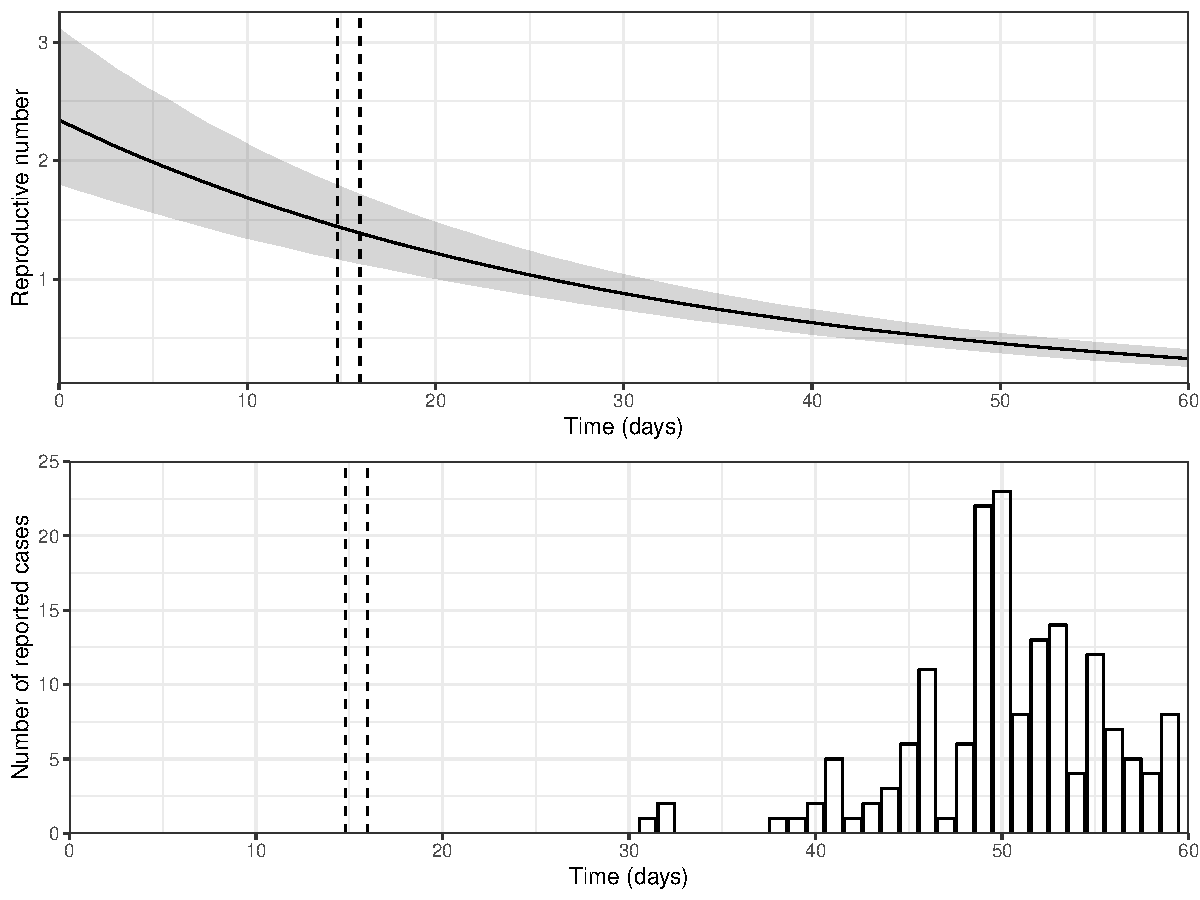
\includegraphics[width=\textwidth]{../figure/mers_time_series.pdf}
\caption{MERS time series. Dashed lines represent 95\% credible intervals of the infection date of the primary date.}
\end{figure}

In figure 1, we present a time series of the outbreak and our estimates of the time varying reproductive number.  
Based on the initial date of infection, we estimate the population-level basic reproductive number to be 1.4 (95\% CI: 1.14 - 1.74).
On the other hand, estimate of the population-level reproductive number at the time of diesase onset of the primary infector is 1.1 (0.92 - 1.3).

\begin{figure}
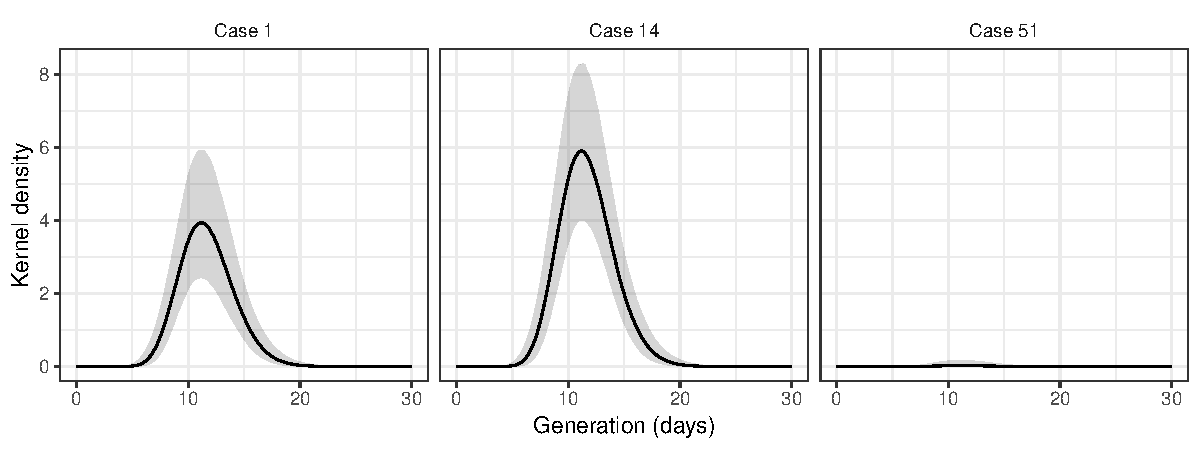
\includegraphics[width=\textwidth]{../figure/kernel.pdf}
\caption{Infection kernels. Case 1 is the primary infector. Case 14 is another superspreader. Case 51 represents an ``average'' infected individual that was represented in the middle of an epidemic but did not infect anyone else.}
\end{figure}

We might be more interested in individual-level kernels due to high heterogeneities observed (Figure 2).
We imposed strong priors on individual varation $\sigma_{\mathcal R}^2$ but we still see fair amount of variation in kernels. Two superspreaders (case 1 infected 26 individuals and case 14 infected 38 individuals based on the incomplete contact tracing) have much stronger kernel compared to case 51, who was chosen as an typical infection.
Individual $\mathcal R$ estimates (integral of the kernel) for case 1 and case 14 are approximately 3.7 and 3; as a comparision, population-level reproductive number at the time of infection of case 14 is 0.95 (95\% CI: 0.78 - 1.12).
With weaker priors, their estimates will be much higher.

\begin{figure}
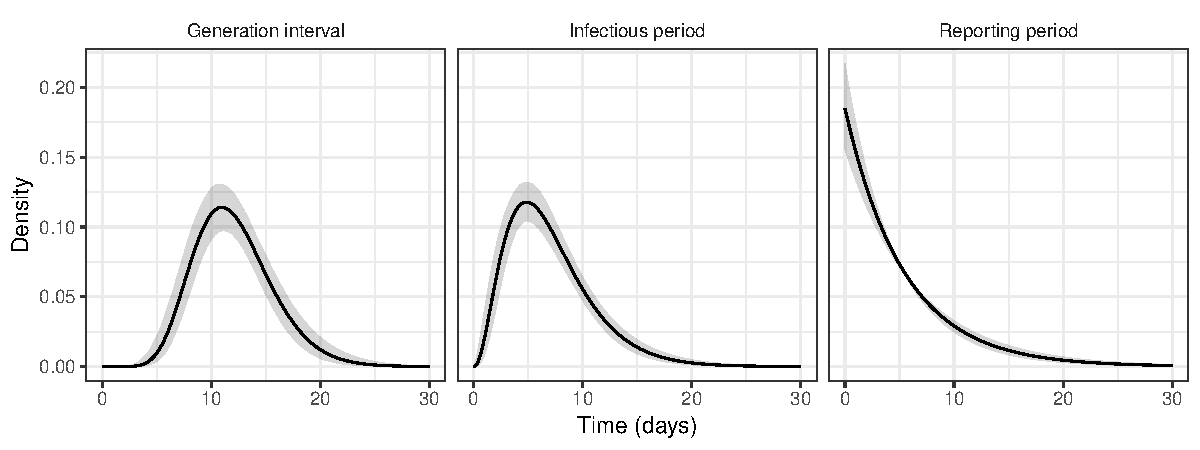
\includegraphics[width=\textwidth]{../figure/distribution.pdf}
\caption{Some distributions.}
\end{figure}

We can also look at distribution of epidemiological periods (Figure 3).
Or even compare generation interval distribution with the observed serial interval distribution (which people often use).

\begin{figure}
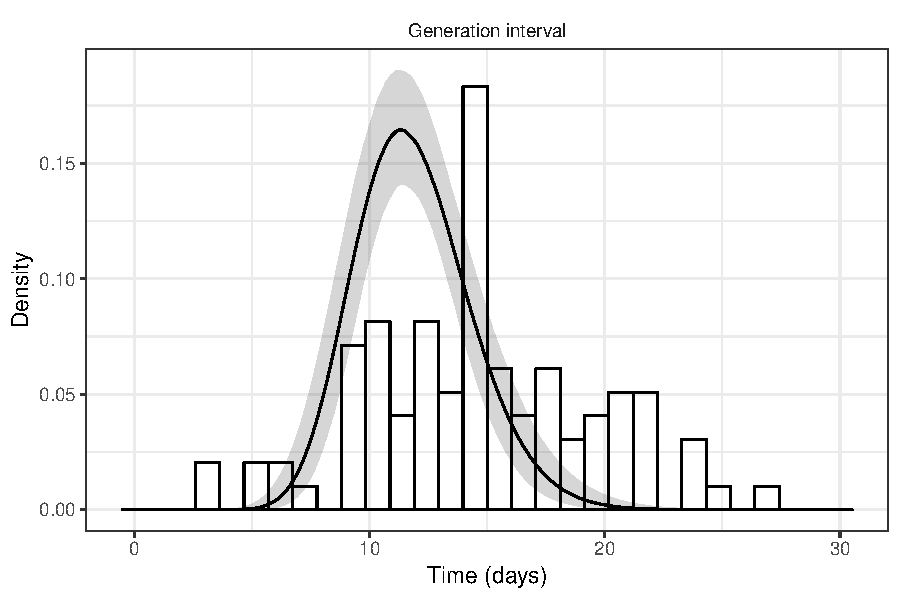
\includegraphics[width=\textwidth]{../figure/generation.pdf}
\caption{Generation-interval distribution (smooth curve) vs obsered serial interval (histogram).}
\end{figure}

\end{document}
